\begin{question}
A random variable $X$ that assumes values in the interval $[0, 1]$ has density function $f(x) = a + b x$,
where $a$ and $b$ are two constants to be determined.

\begin{enumerate}[label={\emph{\alph*})}]
\tightlist
\item Compute $a$ and $b$ such that $f(x)$ has a PDF with probability density in $X = 1$ being the double of the probability density in $X = 0$;
\item compute the quartiles (0.25, 0.5, 0.75 quantiles) of the random variable $X$.
\end{enumerate}
\end{question}

\begin{solution}
\begin{enumerate}[label={\emph{\alph*})}]
\tightlist
\item Given the PDF of the random variable $f(x) = a + bx$ the two constants $a$ and $b$ can be determined by imposing the normalization of the density function and the required conditions at the boundaries:

\begin{equation*}
\begin{cases}
f(1) = 2\cdot f(0)\\
\int_0^1 f(x)dx = 1
\end{cases}  
\end{equation*}
The first equation gives $a+b = 2a \implies a = b$ while the integral can be easily solved

\begin{equation*}
\int_0^1 f(x)dx = \left(ax + \frac{a}{2}x^2\right|^1_0 = 1 \implies a = \frac{2}{3}
\end{equation*}

\item From the first point we fully determined the PDF $f(x) = \frac{2}{3}(1 + x)$. To compute the quartiles it is first necessary to integrate it to get the corresponding CDF 
\begin{equation*}
F(x) = \int_0^{1/4} f(x)dx = \frac{2}{3}\left(x + \frac{1}{2}x^2\right) = \frac{1}{3}x^2 + \frac{2}{3} x  - \frac{1}{4}
\end{equation*}

Then the first quartile ($Q_1$) is given by $F^{-1}(x) = 1/4$ and similarly for the others
\begin{gather*}
\frac{1}{3}x^2 + \frac{2}{3} x  = \frac{1}{4} \\
Q_1 = -1 \pm \frac{3}{2}\sqrt{\frac{7}{9}} = \frac{1}{2}(\sqrt{7} - 2) = 0.3229\\
Q_2 = \dots = 0.5811\\
Q_3 = \dots = 0.8028
\end{gather*}
\end{enumerate}
\end{solution}

\begin{question}
\label{ex:greedy_pig}
The Greedy Pig Game is a simple dice game. It is played with one single die and the goal is to reach 100 points. Each player in turn starts to roll the die, if it results to be in [2, 6] the corresponding points are acquired and the player can decide either to continue to roll or to stop. If a 1 is rolled the player scores a 0 and her turn ends.

\begin{itemize}
\item What is the expected number of points for one roll ?
\item Imagine a player that has collected $k$ points. Compute and draw the expected points obtained with a further roll. What can be concluded from this plot ?
\end{itemize}
\end{question}

\cprotEnv\begin{solution}
The expected number of points for one roll is the weighted average of the possible points [2, 6] (when the die is 1 no points are assigned) with the probability of 1/6.
\begin{ipython}
ex_roll = 0
for i in range(2, 7):
    ex_roll += 1/6*i

print (ex_roll)
\end{ipython}
\begin{ioutput}
3.3333333333333
\end{ioutput}

If the current points of a player are $k$, in computing the expectation, beside the [2, 6]*1/6 terms, it has to be added a $-k\cdot 1/6$ term in case a 1 is rolled (i.e. in this case the total score goes to 0 and the turn ends).
\begin{ipython}
from matplotlib import pyplot as plt

exps = []
for k in range(1, 51):
    exp = -k*1/6
    for i in range(2, 7):
        exp += 1/6*i
    exps.append(exp)

fig = plt.figure(figsize=(10,8))
plt.plot(range(1, 51), exps)
plt.grid(True)
plt.xlabel("current turn points ($k$)")
plt.ylabel("expected points next roll")
plt.show()
\end{ipython}

Figure~\ref{fig:greedy_pig_expec} shows the expected points distribution in the next roll as a function of the current player points. It looks like that when the player has more than 20 points the expectation becomes negative, so it is not anymore convenient to keep rolling. This is a fundamental clue to derive a game strategy: \emph{keeps rolling until you reach 20 points}.

\begin{figure}[htbp]
	\begin{center}
		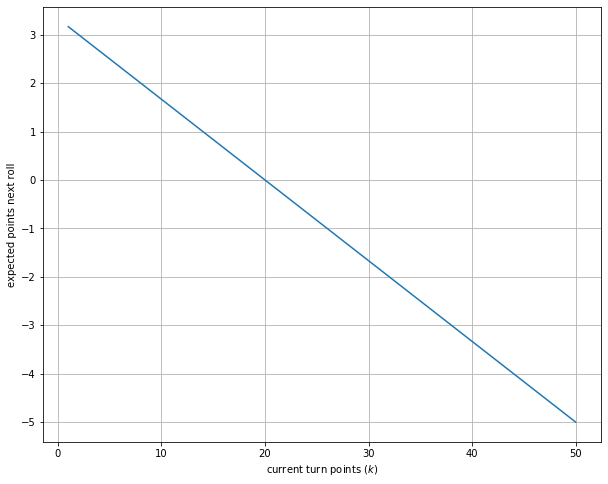
\includegraphics[width=0.7\linewidth]{figures/greedy_pig_expectation}
	\end{center}
\caption{Expected points in the next roll as a function of the current turn points.}
\label{fig:greedy_pig_expec}
\end{figure}
\end{solution}

\begin{question}
Let $X$ be a random variable with density function

\begin{equation*}
f(x) = 
\begin{cases}
k(1 - x^2),~\textrm{if}~0 \leq x \leq 1\\
0,~\textrm{otherwise}		
\end{cases}
\end{equation*}
Find $k$, together with the expectation and the variance of the random variable $Y$ defined as $Y = 3X - 1$.
\end{question}

\cprotEnv\begin{solution}
\label{ex:variance}
To find the value of $k$ we can exploit the normalization condition for a probability density:

\begin{equation*}
\begin{gathered}
\int_\Omega f(x) d\Omega = 1\\
\int_{0}^{1}k(1-x^{2})dx = k\left(x-\frac{1}{3}x^{3}\right|_{0}^{1}= k\left(1-\frac{1}{3}\right) \\
k\left(1-\frac{1}{3}\right) = 1 \implies k = \frac{3}{2}
\end{gathered}
\end{equation*}

The expectation of the variable $Y$ instead equals to
\begin{equation*}
\mathbb{E}[Y] = 3\mathbb{E}[X] - 1
\end{equation*}	
So
\begin{equation*}
\begin{gathered}
\mathbb{E}[X] = \frac{3}{2}\int_{0}^{1}x(1-x^2)dx = \frac{3}{2}\left(\frac{1}{2}x^2-\frac{1}{4}x^{4}\right|_{0}^{1} = \frac{3}{2}\left(\frac{1}{2}-\frac{1}{4}\right) = \frac{3}{8} \\
\mathbb{E}[Y] = 3\cdot\frac{3}{8} - 1 = \frac{1}{8} 
\end{gathered}
\end{equation*}
And finally for the variance:
\begin{equation*}
\begin{aligned}
Var[Y] = & \mathbb{E}[Y^2] - (\mathbb{E}[Y])^2 = \frac{3}{2}\int_{0}^{1}(9x^2 - 6x + 1)(1-x^2)dx - \frac{1}{64} = \\  &\frac{3}{2}\int_{0}^{1}(- 9x^4 + 6x^3 + 8x^2 - 6x + 1)dx - \frac{1}{64} = 
\frac{3}{2}\left(- \frac{9}{5}x^5 + \frac{6}{4}x^4 + \frac{8}{3}x^3 - 3x^2 + x\right|_{0}^{1} - \frac{1}{64} = \\
& \frac{3}{2}\left(- \frac{9}{5} + \frac{6}{4} + \frac{8}{3} - 3 + 1\right) - \frac{1}{64} = \frac{11}{20} - \frac{1}{64} = \frac{171}{320}
\end{aligned}
\end{equation*}

Alternatively it can be demonstrated that the variance of a random variable $Y = a + bX$ can be computed as $Var[Y] = b^2 Var[X]$. Indeed starting from the general form of the variance $Var[Y] = \mathbb{E}[Y^2] - (\mathbb{E}[Y])^2$ and computing each term of the right hand side of the equation 

\begin{equation}
\begin{gathered}
\mathbb{E}[Y^2] = \mathbb{E}[(a+bX)^2] = \mathbb{E}[b^2X^2 + 2abX + a^2] = b^2\mathbb{E}[X^2] + 2ab\mathbb{E}[X]+ a^2  \\
\mathbb{E}[Y]^2 =  (b\mathbb{E}[X] + a)^2 = b^2\mathbb{E}[X]^2 + 2ab\mathbb{E}[X]+ a^2  
\label{eq:each_var}
\end{gathered}
\end{equation}
Substituting Eqs.~\ref{eq:each_var} into the general form of the variance 
\begin{equation}
\begin{gathered}
Var[Y] = b^2\mathbb{E}[X^2] + 2ab\mathbb{E}[X]+ a^2 - (b^2\mathbb{E}[X]^2 + 2ab\mathbb{E}[X]+ a^2) \\ 
= b^2\mathbb{E}[X^2] - b^2\mathbb{E}[X]^2 = b^2 Var[X]
\end{gathered}     
\end{equation}

So $Var[Y] = 9\mathbb{E}[X]$.
\end{solution}

\begin{question}
We want to insure a car of 12000 EUR. The probability that a car is involved in an accident during a year is 0.15 in which case the amount of damage is

\begin{itemize}
\tightlist
\item 20\% of its value with probability 0.8;
\item 60\% of its value with probability 0.12;
\item 100\% of its value with probability 0.08.
\end{itemize}
Find the first annual premium the insurer must charge to have the expected cost of the company equal to 0.
\end{question}

\cprotEnv\begin{solution}
\begin{ipython}
print (f"{0.15 * 12000 * (0.8*0.2 + 0.6*0.12 + 0.08):.2f} EUR")
\end{ipython}
\begin{ioutput}
561.60 EUR
\end{ioutput}
\end{solution}

\begin{question}
The daily expenditure ($X$, in euros) spent by a certain customer in a department store is distributed according to the following density function:

\begin{equation*}
f(x) = 
\begin{cases}
x^2/9000,~\textrm{if}~0 \leq x \leq 30\\
0,~\textrm{otherwise}		
\end{cases}
\end{equation*}

\begin{enumerate}[label={\emph{\alph*})}]
\item calculate the probability that the client has a daily spending between 15 and 20 EUR;
\item what is his/her expected daily expenditure ?;
\item next winter the department store is granting the following "discount vouchers", whose amount depends on the client's expenditure: 1 EUR for spending between 10 and 20 EUR, 1.5 EUR for spending between 20 and 25 EUR,
3 EUR if the expense exceeds 25 EUR. Derive the distribution and the expected value of the discounts obtained by the client.
\item the customer has paid for his/her purchases in the store with a credit card which applies a 4\% charge. What is the probability that the customer has paid (with charges included) between 10 and 15 EUR ?
\end{enumerate}
\end{question}

\cprotEnv\begin{solution}
\begin{enumerate}[label={\emph{\alph*})}]
\tightlist
\item First we need to calculate the CDF by simple integration of the given PDF.
\begin{ipython}
def F(x):
    return x**3/27000

P = F(20) - F(15)
print (P)
\end{ipython}
\begin{ioutput}
0.17129629629629628
\end{ioutput}
\item The expected expense is given by $\int_{0}^{30} xf(x) dx = x^4/36000$
\begin{ipython}
def tot(x):
    return x**4/36000

print (tot(30))
\end{ipython}
\begin{ioutput}
22.5	
\end{ioutput}

\item The expected discount value is given by the weighted average of each discount times the probability of spending the corresponding amount of money:
\begin{ipython}
expected = 1 * (F(20)-F(10)) + 1.5 * (F(25) - F(20)) + 3 * (F(30) - F(25))
print (expected)
\end{ipython}
\begin{ioutput}
1.9467592592592593
\end{ioutput}

\item If the customer spent between 10 and 15 EUR with an extra charge of 4\% (by the usage of the credit card) the real expense limits has to be scaled by $1 - 0.04$, then the corresponding probability can be found using the function \texttt{F}:
\begin{ipython}
xmin = 10*0.96
xmax = 15*0.96
P = F(xmax) - F(xmin)

print (P)
\end{ipython}
\begin{ioutput}
0.07782399999999998
\end{ioutput}
\end{enumerate}
\end{solution}

\cprotEnv\begin{question}
An economist wishes to estimate the total cost of a project. His salary is composed of a fixed part of 12000 EUR plus a variable part of 300 EUR per day of work. The project can be performed between 7 and 11 days, and the economist has derived the following subjective probability distribution for the random variable $X$ (number of days it will take to implement the project):
\begin{ipython}
P = {7:0.10, 8:0.20, 9:?, 10:0.30, 11:0.10}
\end{ipython}
\begin{enumerate}[label={\emph{\alph*})}]
\tightlist
\item What is the probability that the project is carried out in 9 days? Justify your answer.
\item Determine the expected cost of the project and its variance. 
\end{enumerate}
\end{question}

\cprotEnv\begin{solution}
\begin{enumerate}[label={\emph{\alph*})}]
\tightlist
\item Since the assumption is that the work can be completed in between 7 and 11 days, the sum of $P$s has to equal 1. So $P(9)$ can be determined as
\begin{ipython}
P = {7:0.10, 8:0.20, 10:0.30, 11:0.10}
P[9] = 1 - (P[7]+P[8]+P[9]+P[10]+P[11])

print (f"{P[9]:.2f}")
\end{ipython}
\begin{ioutput}
0.30
\end{ioutput}
\item The expected cost of the project results
\begin{ipython}
expected_days = sum([d*p for d, k in P.items()])
E_C = 12000 + 300*expected_days

print (E_C)
\end{ipython}
\begin{ioutput}
14730.0	
\end{ioutput}

Remembering Solution~\ref{ex:variance} the variance in the costs $Var[C]$ (which follows a linear relationship with the number of days $C = 12000 + 300\cdot d$) becomes
\begin{ipython}
var_days = sum([(d**2)*p for d, k in P.items()])
b = 300
print (b**2 * var_days)
\end{ipython}
\begin{ioutput}
116100.0	
\end{ioutput}
\end{enumerate}
\end{solution}

\begin{question}
A casino advertises that the expected prize won by its clients is 600 EUR, with risk $\sigma$ = 360.
\begin{enumerate}[label={\emph{\alph*})}]
\tightlist
\item Calculate the probability that a player wins between 150 and 1050 EUR.
\item How would the above probability change if $\sigma$ = 420 ?
\item What is the probability that the prize won by a player deviates at least 504 EUR from its expectation?
\end{enumerate}
\end{question}

\cprotEnv\begin{solution}
In this case it is safe to assume that the wins are distributed as a Gaussian with mean 600 EUR and standard deviation 360 EUR. 
\begin{enumerate}[label={\emph{\alph*})}]
\tightlist
\item It is much easier to convert the initial distribution to a standard normal (zero mean and unit variance) using the following transformation
\begin{equation*}
x' = \frac{(x - \mu)}{\sigma}
\end{equation*}
in such a way \texttt{scipy.stats.norm} can be used.

\begin{ipython}
from scipy.stats import norm

# convert the two limits in the standard normal
xmin = (150 - 600)/360
xmax = (1050 - 600)/360

print (xmin, xmax)
print (norm.cdf(xmax) - norm.cdf(xmin))
\end{ipython}
\begin{ioutput}
-1.25 1.25
0.7887004526662893
\end{ioutput}

\item If the risk (i.e. uncertainty) increases the probability of winning an amount of money in the same range is expected to decrease. Let's check using the same technique as in the previous answer.
\begin{ipython}
xmin = (150 - 600)/420
xmax = (1050 - 600)/420

print (xmin, xmax)
print (norm.cdf(xmax) - norm.cdf(xmin))
\end{ipython}
\begin{ioutput}
-1.0714285714285714 1.0714285714285714
0.7160232282490884
\end{ioutput}

Indeed now the range has shrunk from $\pm1.5\sigma$ to $\pm1.07\sigma$. 

\item Finally, we can determine the probability that a win exceeds 504 EUR the mean in a similar fashion.

\begin{ipython}
xmin = 504/360

print (xmin)
# the factor 2 because the win can exceed both ways the mean
print (norm.cdf(-xmin) * 2)
\end{ipython}
\begin{ioutput}
1.4
0.16151331846754213
\end{ioutput}
\end{enumerate}
\end{solution}
